\section{Group system}\label{sec:group-system}

One of the requirements for our app was that it should be possible to group repositories together.
The grouping is needed to view statistics for multiple repositories at once and also compare groups of repositories.
The grouping system should be also capable of controlling user access rights to different repositories.

Requirements for grouping system
\begin{itemize}
    \item It shall be possible to group both repositories and groups already consisting of repositories.
    \item Single repository may be possible of multiple groups.
    \item Group access can be limited to only viewing summary (group total).
    \item Granting user an access group subgroups and then removing it shall have no side effects. (Accesses to subgroups shall not be persisted)
\end{itemize}

As the groups may consist of both groups and repositories we decided to automatically create group for every repository.
This means now groups can only consist of zero or more other groups.
If we need te get the repository we can fetch all the group ids that are accessible and then query from repositories database by
comparing repositories group id against previously fetched ids;
To fetch group with all of its subgroups a recursive Structured Query Language (SQL) query was needed as the groups'
hierarchy formulates a tree like structure.
Our database provider PostgreSQL supports recursive queries so there were no technical problems with implementing it on SQL database.
A simplified version of our group system database tables can be seen of Figure~\ref{fig:group_system}

\begin{figure}[h]
    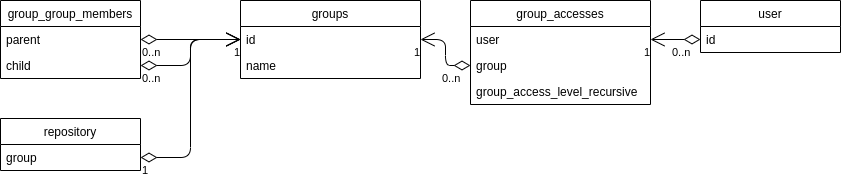
\includegraphics[width=\textwidth]{figures/group_system}
    \caption{Application groups system}
    \label{fig:group_system}
\end{figure}

This tree like groups' hierarchy allows us to easily give and take user access to any group.
If we want to change access from only parent group to also all subgroups access, we can simply toggle access\_level\_recursive
variable.
If we remove one particular group access, all other accesses remain in place, meaning that you some group was accessible
also via some other group access, you still have the access.
